% 图 12.2 —— 手工重建（两面板：大椭圆 = 全集；内椭圆 = 子集；元素点 a/b/c）
%%
%% ══ 按用户意见重做（2026-09-19）══
%%  ①「曲线需要做的更平滑」：原稿是 prims2 拆出来的**折线链** —— 大椭圆被切成
%%     5 段三次贝塞尔 + 3 条直线段，渲染出来左边和顶部有明显折角。
%%     这些本来就是正椭圆，一律改用 `ellipse` 解析画。
%%  ②「字母需要往上放，字母底部的白色背景叠在了曲线上」：标签整体上移（见下）。
%%
%% 参数量法：原书 600dpi 裁切 src_hi/12.2.png（1348x328，1.8070 px/画布单位）。
%%   **不用射线法** —— 右面板两个内椭圆互相重叠，射线「第一条穿墨」会串形
%%   （实测拟成半径 52 的圆，套色一看就错）。
%%   改用**过中心的横/竖剖线**：椭圆上任一过中心的弦都是直径，中点即中心。
%%     横剖 y0 -> x 左右 -> cx ；竖剖 cx -> y 上下 -> cy ；再回代一次即收敛。
%%   墨段取「连续 1 段的中点」= 笔画中心线，所以量到的直接是中心线，不用扣半线宽。
%%   结果与套色图逐条核对过（12_2_fit.png）。
%%
%% 线宽：原书墨迹实测 —— 大椭圆 ≈4.8、内椭圆 ≈4.0（剖线斜切会放大，已按切角折算）。
\documentclass[12pt]{standalone}
\usepackage{fontspec}
\setsansfont{Arial}
\newfontfamily\mfallback{DejaVu Sans}
\usepackage{tikz}
\begin{document}
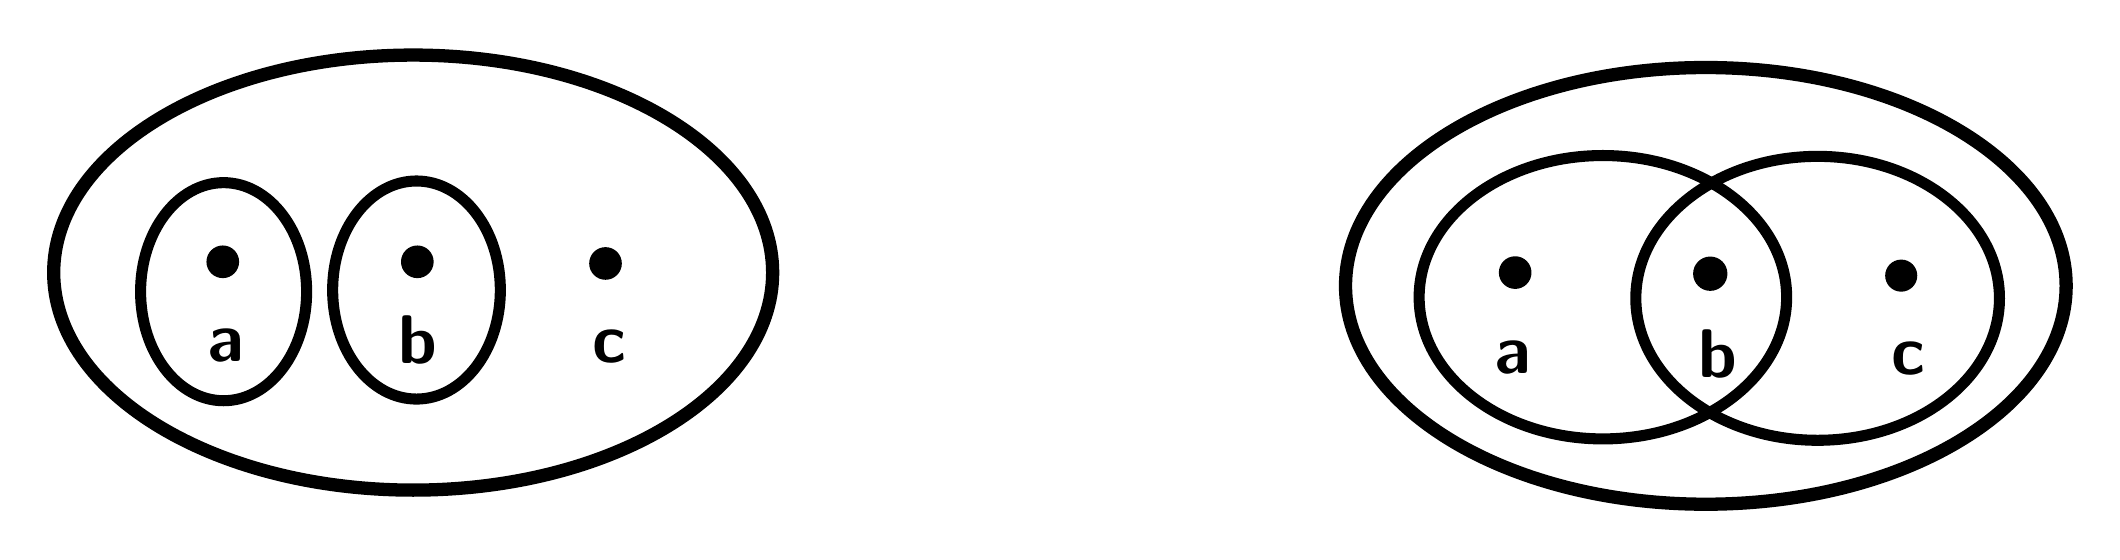
\begin{tikzpicture}[x=1pt, y=-1pt, line width=4.0pt, line cap=round, line join=round]

  %% ════ 大椭圆（= 全集）════
  \draw[line width=4.8pt] (139.3, 88.5) ellipse (129.9 and 78.6);
  \draw[line width=4.8pt] (606.4, 93.3) ellipse (130.2 and 78.9);

  %% ════ 左面板：a、b 各自的子集（互不相交）════
  \draw ( 70.8, 95.4) ellipse (30.0 and 39.4);
  \draw (140.5, 94.8) ellipse (30.3 and 39.4);

  %% ════ 右面板：{a,b} 与 {b,c}（相交，b 落在交里）════
  \draw (569.2, 97.4) ellipse (66.4 and 51.2);
  \draw (646.8, 97.8) ellipse (65.7 and 51.3);

  %% ════ 元素点 ════
  %% ⚠ 原稿的坐标取自 probe，实测**系统性偏了**（y 一律大约 3.6，x 左面板还偏 4~5）。
  %%   这里改为在原图连通域上直接量（面积 250~450 那块就是实心点，21x21 px，圆度 10.34）。
  \fill ( 70.5, 84.6) circle (5.9);
  \fill (140.8, 84.6) circle (5.9);
  \fill (208.8, 85.2) circle (5.9);
  \fill (537.5, 88.5) circle (5.9);
  \fill (608.0, 88.9) circle (6.2);
  \fill (677.0, 89.6) circle (5.8);

  %% ════ 字母 ════
  %% ⚠ 用户指定：本图**不要白底**（字母本来就落在空白处，不会被曲线压到）。
  %% ⚠ **用户说的「字母要往上放」是对的** —— 原稿坐标取自 probe，
  %%   而 probe 在这张图上系统性偏低约 3.5（左面板还偏右 4~5）。
  %%   正解：把每个字母在原图里当**独立连通域**量出字形框（面积 400~2500 那批），
  %%   再把「只画字、不画线」编一版量我自己的字形框，两个中心差回代坐标 ——
  %%   现在 6 个字与原书字形框中心差都 < 0.7 画布单位。
  %%   ⚠ 原稿把右面板的『c』认成了大写 C（字号也只有 24.2）—— 已改回小写 c（31.4）。
  \node[anchor=center,inner sep=0pt,font=\fontsize{32.0}{40.0}\selectfont] at (71.9,114.8) {\textsf{\textbf{\textit{a}}}};
  \node[anchor=center,inner sep=0pt,font=\fontsize{30.0}{37.6}\selectfont] at (141.1,112.8) {\textsf{\textbf{\textit{b}}}};
  \node[anchor=center,inner sep=0pt,font=\fontsize{31.4}{39.3}\selectfont] at (210.2,115.3) {\textsf{\textbf{\textit{c}}}};
  \node[anchor=center,inner sep=0pt,font=\fontsize{32.0}{40.0}\selectfont] at (536.8,119.2) {\textsf{\textbf{\textit{a}}}};
  \node[anchor=center,inner sep=0pt,font=\fontsize{30.7}{38.3}\selectfont] at (610.9,117.9) {\textsf{\textbf{\textit{b}}}};
  \node[anchor=center,inner sep=0pt,font=\fontsize{31.4}{39.3}\selectfont] at (679.6,119.7) {\textsf{\textbf{\textit{c}}}};

  % 钉死画布：否则超出的图元/控制点会把页面撑大，1:1 回比就失准
  \pgfresetboundingbox
  \path[use as bounding box] (0,0) rectangle (746,182);
\end{tikzpicture}
\end{document}
